%%%%%%%%%%%%%%%%%%%%%%%%%%%%%%%%%%%%%%%%%%%%%%
\section{Quasi-elastic Scattering}
%%%%%%%%%%%%%%%%%%%%%%%%%%%%%%%%%%%%%%%%%%%%%%
 In Fig.~\ref{e_scatt}, an electron with known initial energy, $E_{0}$, and final energy, $E'$, interacts with a charged nucleus by exchanging a virtual photon with the four momentum $q=(\nu,\vec{q})$, where the energy transfer $\nu = E_{0}-E'$ and the momentum transfer $\vec{q}=\vec{k}-\vec{k'}$. One can probe the nucleus at different scales by varying $q$. Elastic scattering denotes the process of electrons interacting with the entire nucleus while the nucleus remains intact. Quasielastic (QE) scattering refers to the case where electrons scatter off individual moving nucleons which are ejected from the nucleus thereafter. Fig.~\ref{e_trans} is a schematic of the inclusive electron scattering cross sections as a function of $\nu$~\cite{qe_donal}, where a broad peak is seen for the QE process due to the interval motion of the nucleons. Nucleons can be excited at even larger $\nu$ and resonances start to contribute to the cross section through inelastic scattering. Electrons directly probe the quark properties in the nucleons at very large $\nu$ through deep inelastic scattering (DIS). 
\begin{figure}[!ht]
  \begin{center}         
    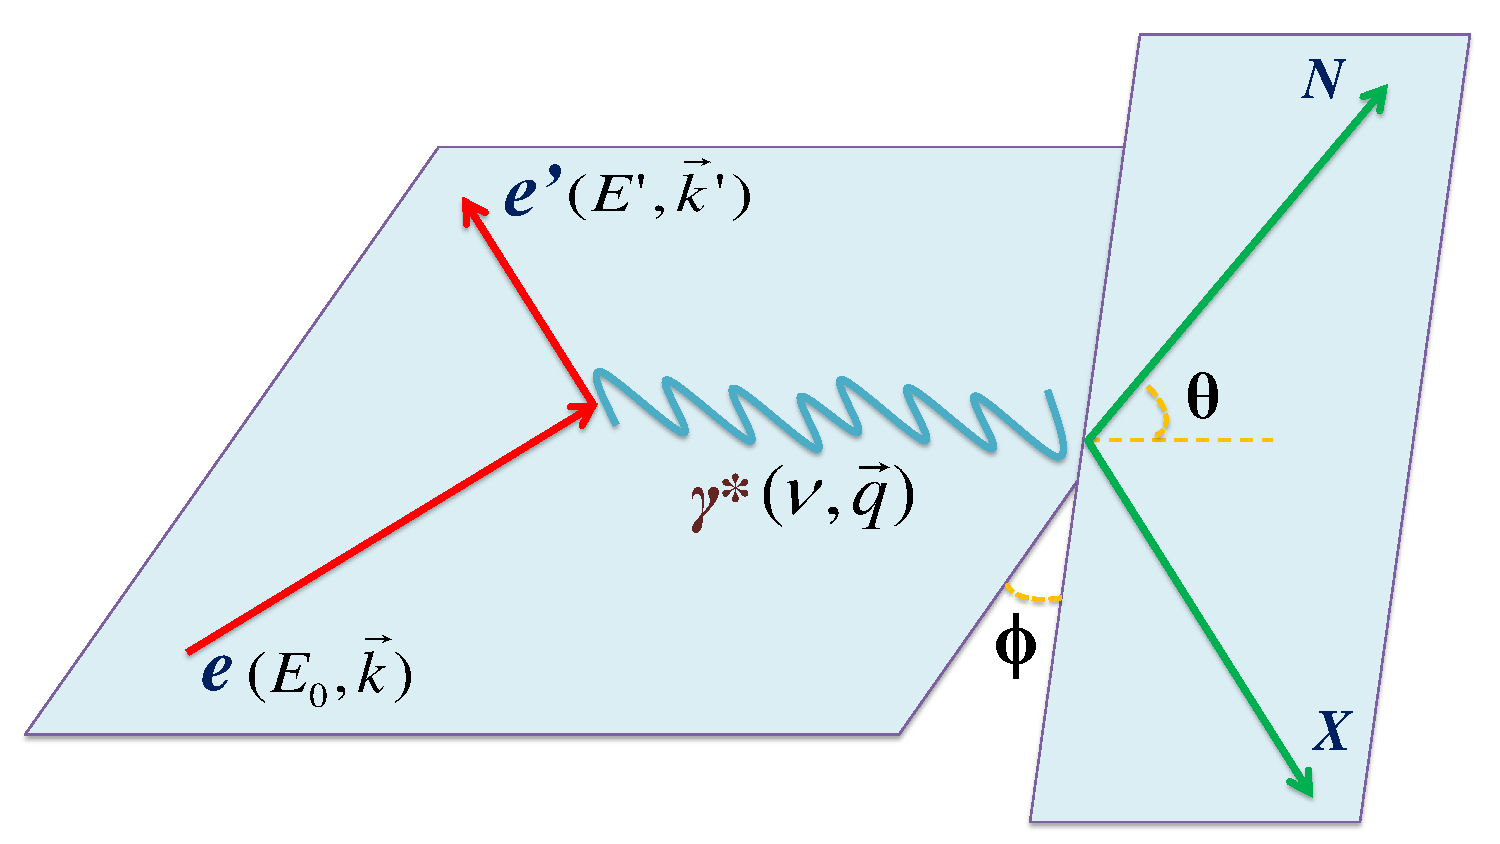
\includegraphics[type=pdf,ext=.pdf,read=.pdf,width=0.60\linewidth]{./figures/physics/e_scatt}
    \caption[Schematic of electron-scattering]{\footnotesize{Schematic of electron-scattering.}}
    \label{e_scatt}
  \end{center}
\end{figure}
\begin{figure}[!ht]
  \begin{center}
    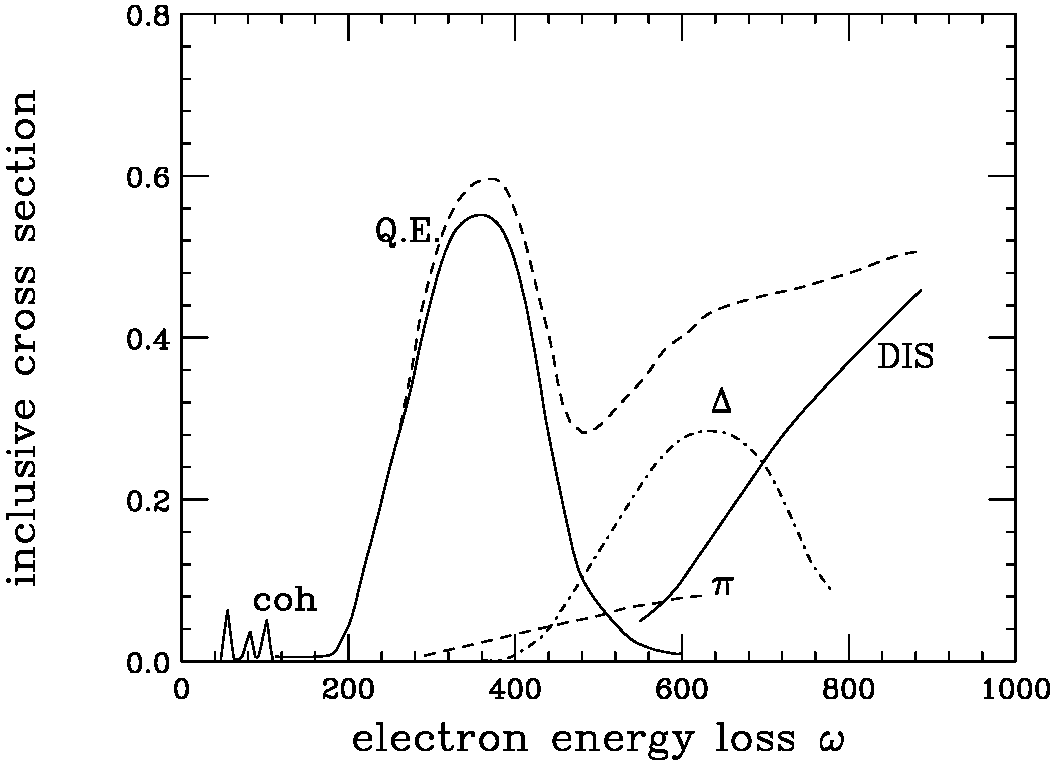
\includegraphics[type=pdf,ext=.pdf,read=.pdf,width=0.60\linewidth]{./figures/physics/eesm}
    \caption[Electron energy transfer]{\footnotesize{Inclusive cross section on the y-axis versus the energy loss $\omega\equiv\nu=E_{0}-E'$ on the x-axis. The Figure is obtained from Ref.~\cite{qe_donal}.}}
    \label{e_trans}
  \end{center}
\end{figure}

A convenient kinematic parameter for identifying these different scattering processes is the Bjorken variable, $x_{bj}=Q^{2}/(2m_{N}\nu)$, which was firstly proposed as a scaling variable to describe DIS from nucleons. It is then interpreted as the momentum fraction of the struck quark. For scattering off a nucleon, $x_{bj}$ goes from 0 to 1, and the elastic peak is found at $x_{bj}=1$. In the case of scattering off a nucleus in QE process, $x_{bj}$ extends to the region of $0<x_{bj}<M_{A}/m_{N}$, where $x_{bj}=1$ is now the location of the QE peak and the nuclear elastic peak moves to $x_{bj}=M_{A}/m_{N}\simeq A$. For convenience, $m_{N}$ is usually replaced by the proton mass during the experimental data analysis, and will be used in the rest of this thesis:
\begin{equation}
  x_{bj} = Q^{2}/(2m_{p}\nu).
  \label{xbj_define}
\end{equation}
  
 In QE scattering, an electron knocks a nucleon out from the nucleus. This provides an opportunity to study the nucleon's original ground state. One can detect the scattered electrons in coincidence with the struck nucleon, and extract the exclusive cross section which contains the initial properties of the nucleon inside the nuclear medium. In the PWIA, the exclusive cross section is the sum of the cross sections of the individual nucleons weighted by the spectral function~\cite{DeForest1983,john_thesis}:
\begin{equation}
  \frac{d^{5}\sigma}{dE'd\Omega d^{3}\vec{p'}} = \sum_{nucleons}\sigma_{eN}\cdot S'_{N}(E_{0},\vec{p}_{0}),
  \label{quasi_xs_spectral_function}
\end{equation}
where $\sigma_{eN}$ is the cross section of electron-nucleon scattering, and $S'_{N}(E_{0},\vec{p}_{0})$ is the nuclear spectral function and gives the probability of removing a nucleon with initial energy $E_{0}$, and momentum $\vec{p}_{0}$ from the target nucleus~\cite{qe_donal}. Within the IPSM, a nucleon moves independently in a mean field, and the spectral function can be written as~\cite{qe_donal}:
\begin{equation}
 S'_{N}(E_{0},\vec{p}_{0}) = \sum_{n\in \lbrace F\rbrace}\vert\phi_{n}(\vec{p}_{0})\vert^{2}\delta(E_{0}-E_{n}),
\end{equation}
where $\phi_{n}(\vec{p}_{0})$ is the wave-function of the nucleon when it is in an eigenstate with the eigen-energy $E_{n}$. The sum is extended to all occupied states within the Fermi sea $\lbrace F\rbrace$. 

%%%%%%%%%%%%%%%%%%%%%%%%%%%%%%%%%%%%%%%%%% 	  
\subsection{Inclusive Cross Section}
%%%%%%%%%%%%%%%%%%%%%%%%%%%%%%%%%%%%%%%%%% 	  
\begin{figure}[!ht]
  \begin{center}
    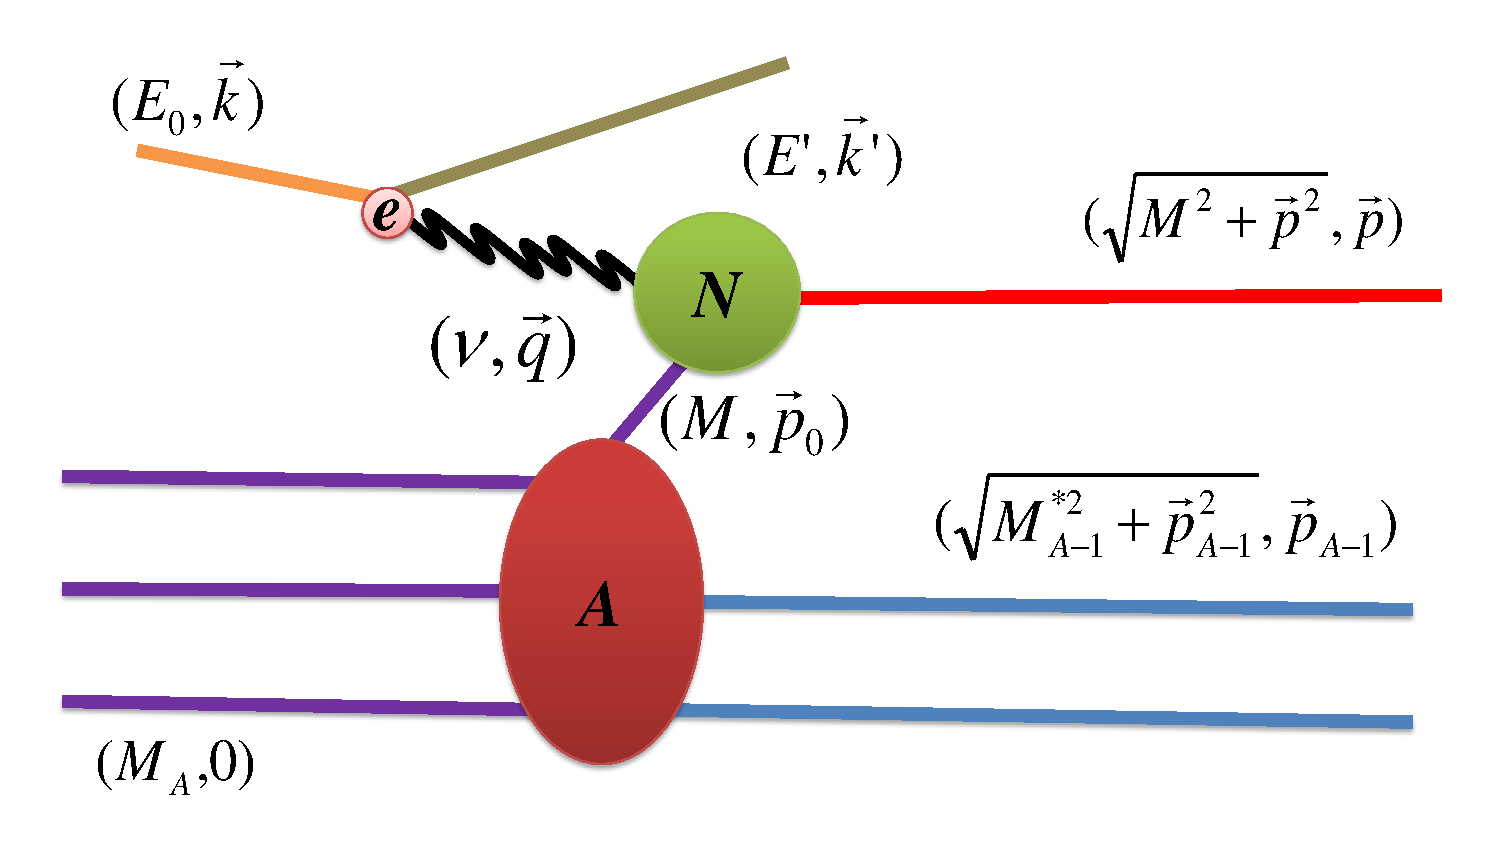
\includegraphics[type=pdf,ext=.pdf,read=.pdf,width=0.60\linewidth]{./figures/physics/includ_diagram}
    \caption[Schematic of QE electron scattering]{\footnotesize{Schematic of QE electron scattering where $\vec{p}_{A-1} = -\vec{p}_{0}$ for fixed targets.}}
    \label{qe_scatt_diag}
  \end{center}
\end{figure}
 In inclusive electron-nucleus QE scattering (Fig.~\ref{qe_scatt_diag}), the cross section is determined by only detecting the scattered electron with the four momentum, ($E'$, $\vec{k'}$). The knocked out nucleons with ($\sqrt{M^{2}+ \vec{p}^{2}}$, $\vec{p}$), and the potentially excited ($A-1$) recoil system in the final state ($\sqrt{M_{A-1}^{*2}+ \vec{p}_{A-1}^{2}}$, $\vec{p}_{A-1}$) are undetected. To obtain the inclusive cross section from Eq.~\eqref{quasi_xs_spectral_function}, one separates the contributions from protons and neutrons, and integrates over the final states of the nucleons:
\begin{equation}
  \frac{d^{3}\sigma}{dE'd\Omega} = \int (Z\sigma_{ep}S'_{p}(E_{0},\vec{p}_{0})+N\sigma_{en}S'_{n}(E_{0},\vec{p}_{0})) d^{3}\vec{p},
\end{equation}
where the subscripts in $dE'_{e}d\Omega_{e}$ have been omitted since only electrons are measured.

Assuming the spectral function is spherically symmetric and the difference in the spectral function of protons and neutrons can be ignored, a more general form $S'(E_{0},p_{0})$ can be factored out from the equation. Since $\vec{p} = \vec{p}_{0}+\vec{q}$, where $\vec{q}$ is fixed when measuring $E_{0}$ and $E'$, one can replace $d^{3}\vec{p}$ by $d^{3}\vec{p}_{0}$. In spherical coordinates, $d^{3}\vec{p}_{0}=p_{0}^{2} dp_{0}d(cos\theta) d\phi$, and the cross section becomes:
\begin{equation}
  \frac{d^{3}\sigma}{dE'd\Omega} = 2\pi \int \tilde{\sigma}_{0}\cdot S'(E_{0},p_{0})\cdot p_{0}^{2}dp_{0}d(cos\theta),
  \label{in_xs_org}
\end{equation}
where
\begin{equation}
  \tilde{\sigma}_{0} = \frac{1}{2\pi}\int_{0}^{2\pi} \left( Z\sigma_{ep}+N\sigma_{en} \right)d\phi.
\end{equation}

Eq.~\eqref{in_xs_org} can be further simplified by considering energy conservation. From Fig.~\ref{qe_scatt_diag}, for a fixed target, $\vec{p}_{A-1} = - \vec{p}_{0}$, which gives: 
\begin{equation}
  M_{A}= E_{0}+ \sqrt{M_{A-1}^{*2}+p_{0}^{2}},
  \label{eqma_e0}
\end{equation}
and,
\begin{equation}
  \quad  M_{A}+\nu = \sqrt{M^{2}+(\vec{p}_{0}+\vec{q})^{2}}+\sqrt{M_{A-1}^{*2}+p_{0}^{2}},
  \label{ene_mom_cons}
\end{equation}
where $M$ and $M_{A}$ are the mass of the ejected nucleon and the target nucleus, respectively. $M_{A-1}^{*}$ is the mass of the recoiling $(A-1)$ system, where the superscript * denotes that it could be in an excited state. Combining Eq.~\eqref{eqma_e0} and Eq.~\eqref{ene_mom_cons}, one has:
\begin{equation}
 E_{0} + \nu = \sqrt{M^{2}+p_{0}^{2}+q^{2}+2p_{0}qcos\theta}.
\end{equation}
Since $\vec{q}$ and $\nu$ are fixed, $E_{0}$ can be determined by $p_{0}$ and $cos\theta$. One defines a $\delta$-function, $\delta(E_{0}+\nu-\sqrt{M^{2}+p_{0}^{2}+q^{2}+2p_{0}qcos\theta})$, and inserts it into the integral:
\begin{equation}
  \frac{d^{3}\sigma}{dE'd\Omega} = 2\pi \int \tilde{\sigma}_{0}\cdot S'(E_{0},p_{0})\cdot \delta \cdot p_{0}^{2}dp_{0}d(cos\theta)dE_{0}.
  \label{in_xs_org2}
\end{equation}
Integrating over $cos\theta$, one rewrites the formula as follows~\cite{john_thesis}:
\begin{equation}
  \frac{d^{3}\sigma}{dE'd\Omega} = 2\pi \int \tilde{\sigma}_{0}\cdot \frac{E_{N}}{p_{0}q} \cdot S'(E_{0},p_{0})\cdot p_{0}^{2}dp_{0}dE_{0},
\end{equation}
where $E_{N}=\sqrt{M^{2}+p^{2}}$ denotes the energy of the struck nucleon.

One can define the separation energy, $E_{s}\equiv M_{A-1}^{*}+M-M_{A}$, and considering Eq.~\eqref{eqma_e0}, the spectral function becomes $S(E_{s},p_{0})dE_{s}\equiv - S'(E_{0},p_{0})dE_{0}$ through the Jacobian transformation~\cite{john_thesis}. By defining $\tilde{\sigma}=\tilde{\sigma_{0}}\cdot E_{N}/q$, the cross section is rewritten as:
\begin{equation}
  \frac{d^{3}\sigma}{dE'd\Omega} = 2\pi \int_{E_{s}^{min}}^{E_{s}^{max}} \int_{p_{0}^{min}}^{p_{0}^{max}}\tilde{\sigma}\cdot S(E_{s},p_{0})\cdot p_{0}dp_{0}dE_{s},
  \label{in_qe_xs1}
\end{equation}
where $p_{0}^{min}$ and $p_{0}^{max}$ can be obtained from Eq.~\eqref{ene_mom_cons} when $\vec{p}_{0}$ and $\vec{q}$ are parallel:
\begin{equation}
  \quad  M_{A}+\nu = \sqrt{M^{2}+y^{2}+2yq+q^{2}}+\sqrt{M_{A-1}^{*2}+y^{2}}.
  \label{ene_mom_cons_y}
\end{equation}	
Two solutions, $y_{1}$ and $y_{2}$ ($y_{1}<y_{2}$), give the values of $p_{0}^{min}$ and $p_{0}^{max}$, respectively. $E_{s}^{min}$ corresponds to the minimum separation energy when the recoil nucleus is in its ground state. $E_{s}^{max}$ is the maximum separation energy when the struck nucleon is at rest in the final state, i.e. $p_{0}^{min}(E_{s}^{max}) = p_{0}^{max}(E_{s}^{max})$, and it can be given as:
\begin{equation}
  E_{s}^{max}=\sqrt{(M_{A}+\nu)^{2}-q^{2}}-M_{A}.
\end{equation}
%%%%%%%%%%%%%%%%%%%%%%%%%%%%%%%%%%%%%%%%%%%%%%%%%%%%%%%%%%%%%%%%%%%
\subsection{Momentum Distribution and y-Scaling}
%%%%%%%%%%%%%%%%%%%%%%%%%%%%%%%%%%%%%%%%%%%%%%%%%%%%%%%%%%%%%%%%%%%
 The integral of the spectral function over the separation energy leads to the momentum distribution:
\begin{equation}
  n(p_{0}) = \int_{E_{s}^{min}}^{\infty} S(E_{s},p_{0})dE_{s},
  \label{np_mom_eq}
\end{equation}
which is one of the two main properties of nuclei, along with the nuclear density, and is directly connected to the many-body wave-function. By understanding the momentum distribution, one has an opportunity to examine the effect of the nuclear medium and the NN interactions. For example, one can study the momentum distribution above the Fermi momentum, $k>k_{F}$, where the mean field contribution vanishes, and probe the short-distance properties of the NN interaction, i.e. SRC.

\begin{figure}[!ht]
  \begin{center}
    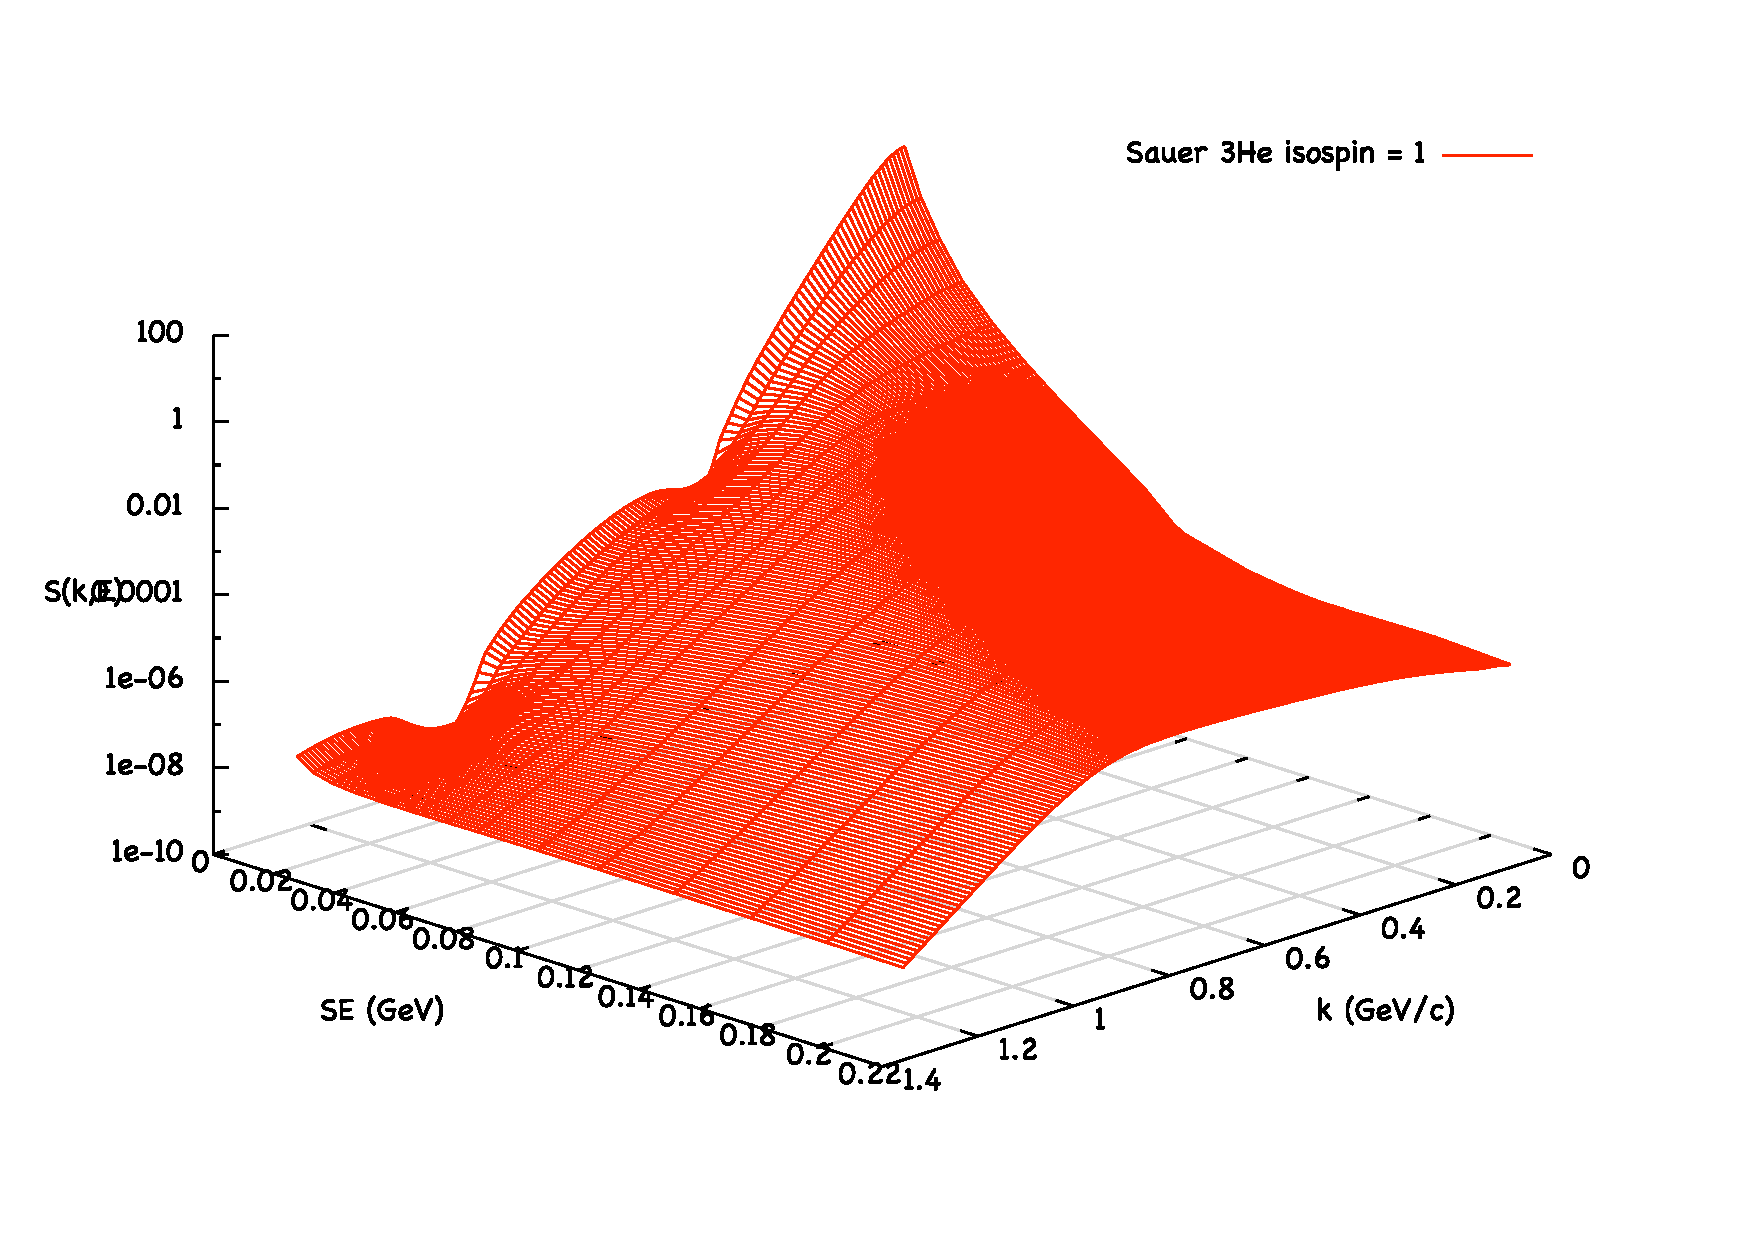
\includegraphics[type=pdf,ext=.pdf,read=.pdf,width=0.70\linewidth]{./figures/physics/3HeSKETeq1}
    \caption[Spectral function for $\mathrm{^{3}He}$]{\footnotesize{Spectral function for $\mathrm{^{3}He}$ as a function of the separation energy $E_{s}$ (given as $SE$ here) and the initial momentum $p_{0}$ (given as $k$ here) for the process of knocking out a nucleon from the nucleus. The magnitude of the spectral function decreases at large values of $E_{s}$ and $p_{0}$, so the upper limits of the double integrals in Eq.~\eqref{in_qe_xs2} can be approximately extended to infinity. Plot was provided by Ref.~\cite{donal_prvt}.}}
    \label{pkem}
  \end{center}
\end{figure}
 However, as the spectral function, the momentum distribution is also not an experimental observable and can not be directly measured from the electron-scattering experiments. Instead, one studies the y-scaling behaviour~\cite{West1975263,day_arns, PhysRevC.41.R2474, Boffi19931} of inclusive QE scattering and extracts the momentum distribution from the scaling function which is directly related to the measured cross sections.

 Because the spectral function decreases rapidly by orders of magnitude toward $E_{s}^{max}$ and $p_{0}^{max}$ (see Fig.~\ref{pkem}), the upper limits of the two integrals in Eq.~\eqref{in_qe_xs1} can be extended to infinity. Meanwhile, $\tilde{\sigma}$ changes very slowly as a function of $E_{s}$ and $p_{0}$, so it can be factored out from the integral and evaluated at the maximum value of the spectral function at $E_{s}=E_{s}^{0}$. Hence Eq.~\eqref{in_qe_xs1} can be rewritten as:
\begin{equation}
  \frac{d^{3}\sigma}{dE'd\Omega} = 2\pi \bar{\sigma}\int_{E_{s}^{min}}^{\infty} \int_{p_{0}^{min}}^{\infty}S(E_{s},p_{0})\cdot p_{0}dp_{0}dE_{s},
  \label{in_qe_xs2}
\end{equation}
where $\bar{\sigma} \propto \tilde{\sigma}(E_{s}^{0},p_{0}^{min})$~\cite{PhysRevB.36.1208}. 

%%%%%%%%%%%%%%%%%%%%%%%%%%%%%%%%%%%%%%%%%% 	  
%\subsection{y-Scaling}
%%%%%%%%%%%%%%%%%%%%%%%%%%%%%%%%%%%%%%%%%% 	  
 The scaling function can be defined as:
\begin{equation}
  F(y,q) = 2\pi\int_{E_{s}^{min}}^{\infty} \int_{|y|}^{\infty}S(E_{s},p_{0})\cdot p_{0}dp_{0}dE_{s},
  \label{fy_scaling_eq}
\end{equation}
where the new variable, $y$, is defined as the minimum values of momentum in Eq.~\eqref{ene_mom_cons}, $p_{0}^{min}=|y|$, when the $A-1$ system is in its ground state:
\begin{equation}
  M_{A}+\nu = \sqrt{M^{2}+q^{2}+y^{2}+2yq}+\sqrt{M_{A-1}^{2}+y^{2}}.
  \label{y_enegy_conserv}
\end{equation} 

 The validity of the y-scaling in QE region relies on several assumptions: (i) the final state interaction (FSI, see next section) is small at large momentum transfer; (ii) the DIS contribution can be subtracted or ignored; (iii) since $\mathrm{E_{s}}$ and $\mathrm{p_{0}}$ are limited to the finite ranges during the cross section measurements , the error made by extending the upper limit of Eq.~\eqref{fy_mom_eq} to infinity can be neglected; (v) the (A-1) recoil system has to be minimally excited so that the lower limit ($p_{0}^{min}=|y|$) can be treated as independent of $E_{s}$.

If the assumptions above are valid and only the nucleonic degrees of freedom are considered, the scaling function can be treated as independent of $q$ at large momentum transfer~\cite{Boffi19931}, i.e. $F(y,q)\equiv F(y)$. From Eq.~\eqref{in_qe_xs2}, the scaling function can be extracted from the experimental electron-nucleus scattering cross section, $\sigma_{EX}$:
\begin{equation}
  F(y)=\frac{d^{3}\sigma_{EX}}{dE' d\Omega } \frac{1}{Z\sigma_{p}+N\sigma_{n}} \frac{q}{\sqrt{M^{2}+(y+q)^{2}}}.
  \label{fy_scaling_eq2}
\end{equation}
\begin{figure}[!ht]
  \begin{center}
    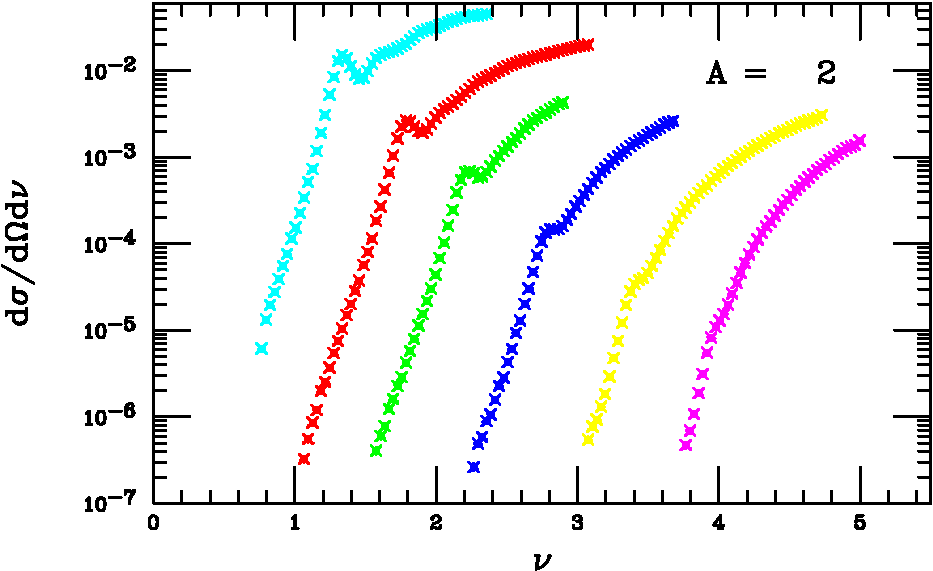
\includegraphics[type=pdf,ext=.pdf,read=.pdf,width=0.80\linewidth]{./figures/physics/xemdeutcs}
    \caption[Deuteron inclusive cross section]{\footnotesize{Deuteron inclusive cross sections~\cite{PhysRevLett.108.092502}. Symbols are experiment data from the E02-019~\cite{nadia_thesis}. From left to right, the $\mathrm{Q^{2}}$ values for different distributions are 2.5 (light-blue), 3.3 (red), 4.1 (green), 5.2 (blue), 6.5 (yellow) and 7.4 (purple) $\mathrm{GeV^{2}}$, respectively. The cross section distributions clearly show the strong $\mathrm{Q^{2}}$ dependence.}}
    \label{nadia_cs_deut}
  \end{center}
\end{figure}
 \begin{figure}[!ht]
  \begin{center}
    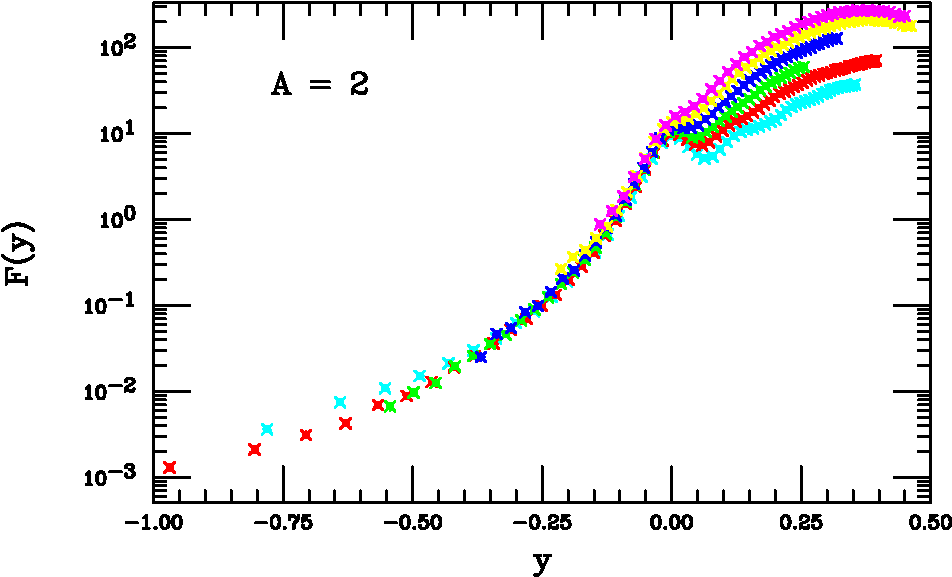
\includegraphics[type=pdf,ext=.pdf,read=.pdf,width=0.80\linewidth]{./figures/physics/xemdeutfy}
    \caption[Scaling function $F(y)$ for deuteron]{\footnotesize{Scaling function $F(y)$ for deuteron~\cite{PhysRevLett.108.092502}. Symbols are experiment data from the E02-019~\cite{nadia_thesis}. The $\mathrm{Q^{2}}$ values for different distributions are 2.5 (light-blue), 3.3 (red), 4.1 (green), 5.2 (blue), 6.5 (yellow) and 7.4 (purple) $\mathrm{GeV^{2}}$, respectively. At $y<0$, the $F(y)$ distributions show much less $\mathrm{Q^{2}}$ dependence for data with high $\mathrm{Q^{2}}$, where the FSI is small. At $y\ge 0$, the distributions are dominated by the DIS processes so the y-scaling is largely violated. Figure is from Ref.~\cite{nadia_thesis}.}}
    \label{y_scaling_deut}
  \end{center}
\end{figure}

As shown in Fig.~\ref{nadia_cs_deut}, the deuteron inclusive cross sections, measured in the E02-019~\cite{nadia_thesis}, reveal a strong $\mathrm{Q^{2}}$ dependence. However, in Fig.~\ref{y_scaling_deut}, the $F(y)$ distributions extracted from these cross sections are only modestly dependent on $\mathrm{Q^{2}}$ at $y<0$, especially at large $\mathrm{Q^{2}}$ ($>3~GeV^{2}$). At modest $\mathrm{Q^{2}}$ ($< 2 GeV^{2}$), the y-scaling starts to be violated due to the FSI. The $F(y)$ fails to scale at $y\ge 0$ where the DIS contributions dominate. The result supports the assumption of y-scaling in QE region.

By reversing the order of the integration in Eq.~\ref{fy_scaling_eq} and based on Eq.~\eqref{np_mom_eq}, $F(y)$ can be rewritten as:
\begin{equation}
  F(y) = 2\pi\int_{|y|}^{\infty}n(p_{0})\cdot p_{0}dp_{0}.
  \label{fy_mom_eq}
\end{equation} 
Hence the momentum distribution can be extracted experimentally from the $F(y)$ distribution~\cite{qe_donal}:
\begin{equation}
  n(p_{0}) = \frac{-1}{2\pi p_{0}}\frac{dF(p_{0})}{dp_{0}} \mid_{p_{0}=|y|}.
  \label{mom_dis_fy}
\end{equation}

\begin{figure}[!ht]
  \begin{center}
    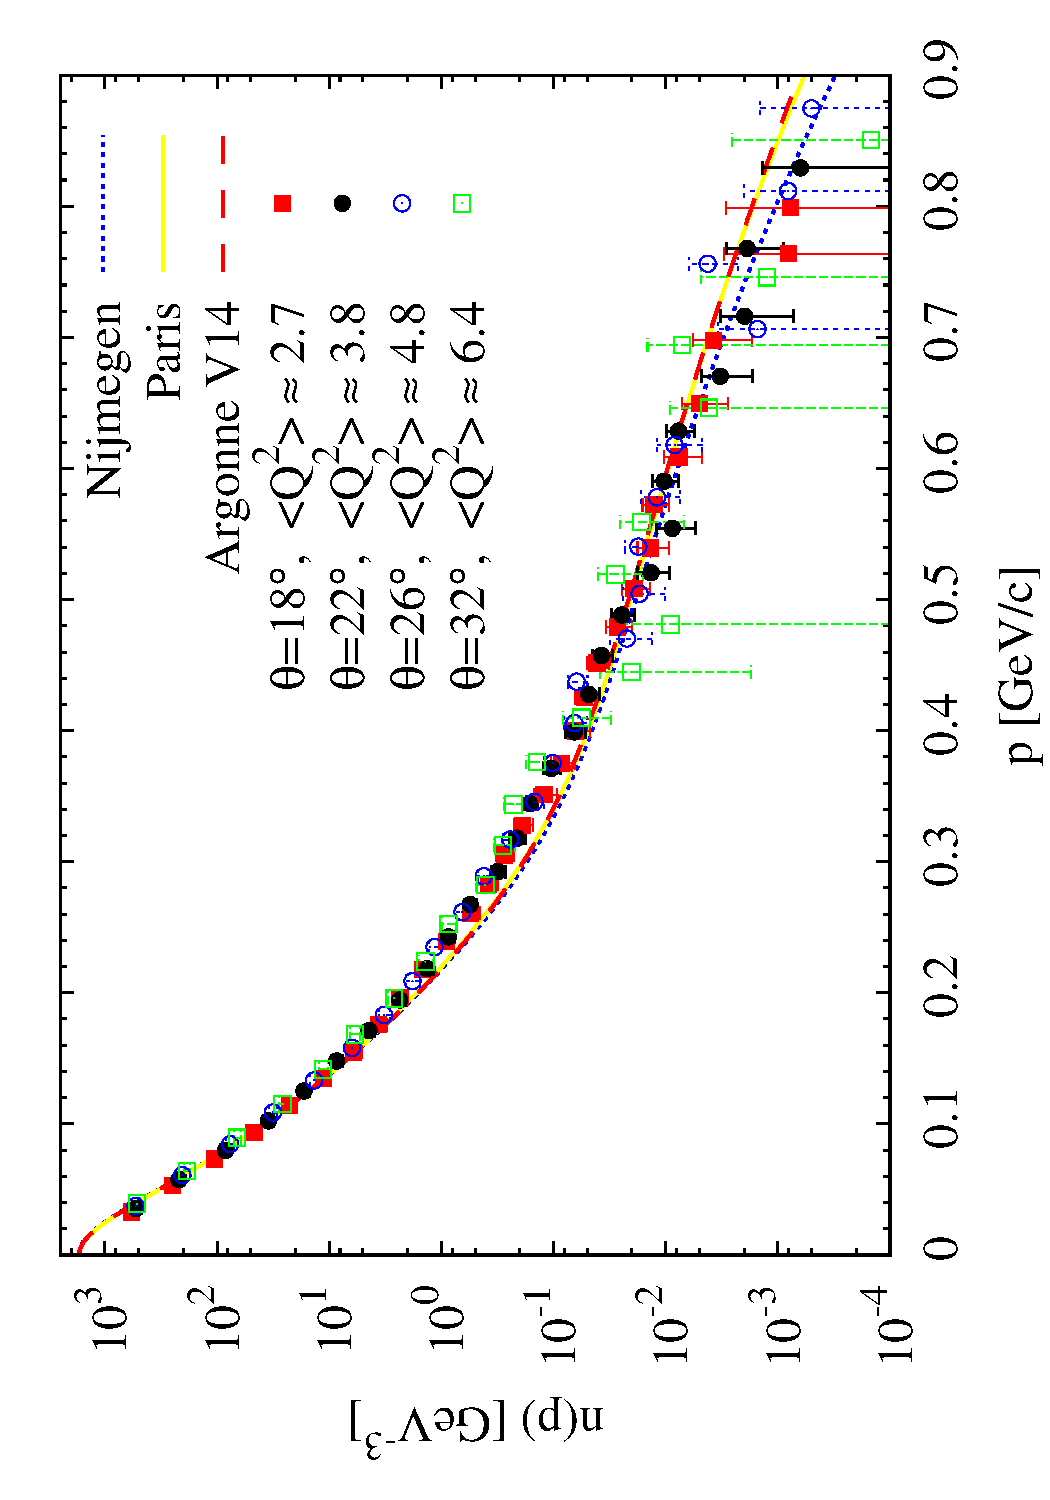
\includegraphics[type=pdf,ext=.pdf,read=.pdf,angle=270,width=0.80\linewidth]{./figures/physics/SRC11_d_nk}
    \caption[Momentum distribution $n(p_{0})$ for deuteron]{\footnotesize{Momentum distribution $n(p_{0})$ for deuteron extracted from the E02-019 data~\cite{nadia_thesis,PhysRevLett.108.092502}, where in this figure, $p_{0}\rightarrow p$. Symbols show the data at different $\mathrm{Q^{2}}$ where the $\mathrm{Q^{2}}$ values are different with ones in the previous two plots since they were quote at different $x_{bj}$ value for other purposes. Lines give the calculations with three different potential models~\cite{PhysRevC.49.2950,Lacombe1981139, PhysRevC.51.38}. Figure is from Ref.~\cite{PhysRevLett.108.092502}.}}
    \label{mom_dis_deut}
  \end{center}
\end{figure}
Eq.~\eqref{mom_dis_fy} provides a way to obtain the nucleon's momentum distribution in the nucleus since $F(y)$ can be directly extracted from the inclusive QE scattering cross section. Fig.~\ref{mom_dis_deut} shows the momentum distribution for the deuteron extracted from the experiment data taken in the $x_{bj}>1$ region along with theoretical calculations derived from various NN potentials~\cite{nadia_thesis,PhysRevLett.108.092502}. From this plot, one can draw the conclusion that studying y-scaling at high $\mathrm{Q^{2}}$ allows the experimental data to be compared with theory in a productive way.

%%%%%%%%%%%%%%%%%%%%%%%%%%%%%%%%%%%%%%%%%% 	  
\subsection{Final State Interaction}
%%%%%%%%%%%%%%%%%%%%%%%%%%%%%%%%%%%%%%%%%%
\begin{figure}[!ht]
  \begin{center}
    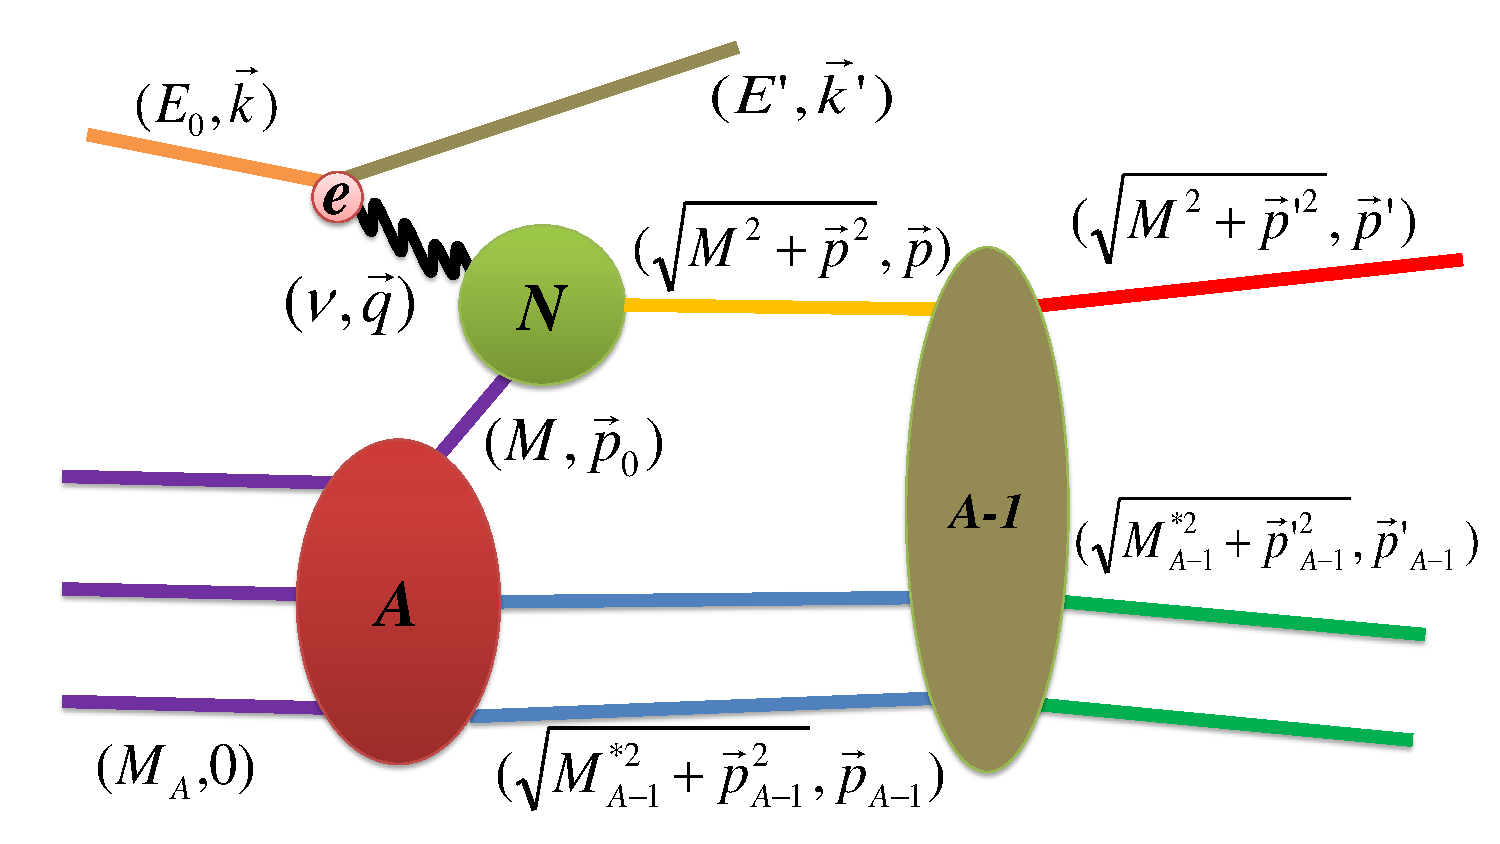
\includegraphics[type=pdf,ext=.pdf,read=.pdf,width=0.80\linewidth]{./figures/physics/FSI}
    \caption[Final state interaction]{\footnotesize{General diagram of final state interaction. The struck nucleon is re-scattered by the $A-1$ system and its final momentum is modified.}}
    \label{fsi}
  \end{center}
\end{figure}
 The FSI effect in the y-scaling has been mentioned above. The FSI refers to the effect of the struck nucleon being re-scattered by the $A-1$ recoil system as it escapes from the nucleus. In the PWIA, nucleons in the nucleus are treated as individual constituents and the spatial resolution of the electron probe is approximately $1/q$. Hence, in the inclusive cross section measurement at large $\mathrm{Q^{2}}$, the FSI is expected to be small (Fig.~\ref{y_scaling_deut}), based on the fact that the interaction time between the virtual photon and the struck nucleon is significantly smaller than the one between the struck nucleon and the recoil system.

However, comparisons between the theoretical calculations and experimental results~\cite{PhysRevC.46.1045,PhysRevC.87.024606} suggest that violations of y-scaling for heavy targets exist. It indicates that the FSI still plays a significant role even at large $\mathrm{Q^{2}}$. Thus, further studies of the FSI contributions for QE scattering at large $\mathrm{Q^{2}}$ are still important.
